%%
%% Copyright (c) 2018-2019 Weitian LI <liweitianux@sjtu.edu.cn>
%% Creative Commons BY 4.0
%%

\chapter{基于深度学习的再电离信号分离新算法}
\label{chap:cdae}

为了能够从强烈的前景干扰中分离出微弱的 EoR 信号,
传统的\ac{fg-rm}方法都依赖于一个关键的前提:
前景干扰具有非常光滑的频谱,而 EoR 信号沿频率维度发生剧烈变化,
两者具有显著不同的频谱结构,从而能够被有效地分离开 \cite{morales2010,chapman2016}.
然而,在实际情况中,未分辨的或者未完全扣除的干扰源在干涉阵列的波束效应的影响下,
会在频率维度产生震荡形式的辐射,破坏前景频谱的光滑性 \cite{liu2009ps}.
这会显著削弱前景干扰与 EoR 信号的可分性,
导致传统\ac{fg-rm}方法的效果大打折扣甚至失效,
因此需要研发能够克服波束效应的 EoR 信号分离新算法.


%=====================================================================
\section{波束的频率依赖效应}
\label{sec:beam-effect}

\begin{figure}[htp]
  \centering
  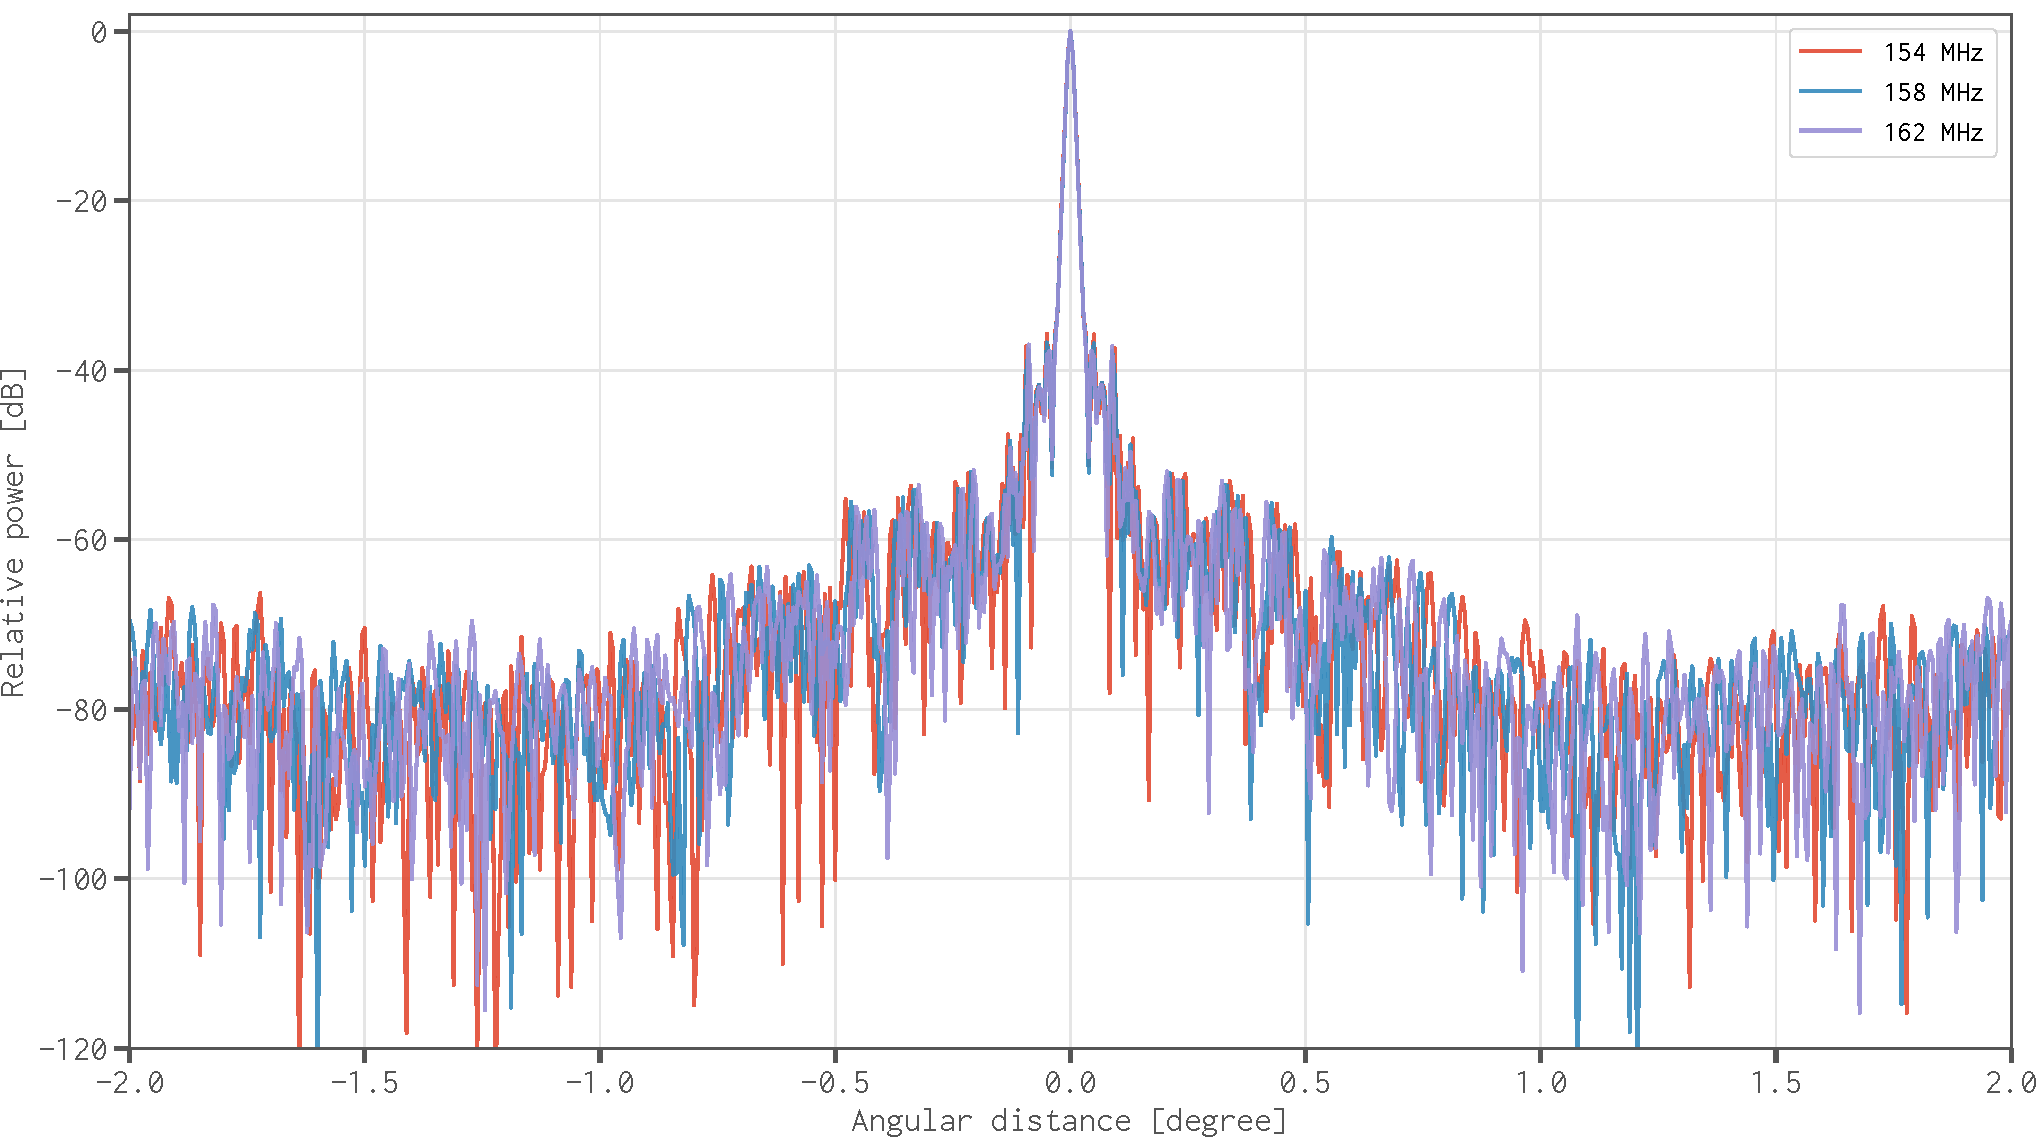
\includegraphics[width=\textwidth]{SKA1-low-psf}
  \bicaption[模拟的 SKA1-Low 综合波束]{%
    在 154、158 和 162 MHz 处模拟的 SKA1-Low \acs*{beam-synthesized}.
    积分时间为 \SI{6}{\hour}.
  }{%
    The simulated synthesized beams of SKA1-Low at 154, 158, and 162 MHz.
    The integration time is \SI{6}{\hour}.
  }
  \label{fig:ska-psf}
\end{figure}

一个干涉阵列拥有的\ac{baseline}的数目和长度均是有限的,
在观测中能实现的 $uv$ 覆盖也是有限而且不完备的 (\autoref{sec:uv-coverage}),
因此,干涉阵列的\ac{beam-synthesized}的形状非常复杂.
如\autoref{fig:ska-psf} 所示,
除了中间一个很窄的\ac{mainlobe},\ac{beam-synthesized}还包含一系列\ac{sidelobe}.
这些\ac{sidelobe}的数量非常多,相对幅度约为 \numrange{0.01}{0.1}\%,
一直延伸到远超出视场的位置.
另见 \citeay{liu2009ps} 的图 1 和图 3.

另一方面,\ac{beam-synthesized}的形状还依赖于观测频率.
\ac{sidelobe}的位置 $\theta$ 会随着频率 $\nu$ 的增大而向中间移动,
即 $\theta \propto \nu^{-1}$.
因此,一个干扰源在视场中所产生的辐射的位置也随频率而变化.
由于仪器的热噪声水平、成像的天区大小、CLEAN 的深度等因素的限制,
视场中总是存在一批未分辨的以及未完全扣除而残留的干扰源.
由这些干扰源的辐射综合而成的前景干扰,
在频率维度将出现类似\ac{beam-synthesized}的\ac{sidelobe}形状的起伏.
这将破坏前景辐射的频谱光滑性,使得前景干扰具有类似 EoR 信号的小尺度频谱结构,
导致传统\ac{fg-rm}方法无法有效地将两者区分开.
另见 \citeay{liu2009ps} \S\,1.


%=====================================================================
\section{基于深度学习的新算法}

鉴于\ac{beam-synthesized}的形状非常复杂,并且随频率和位置而变化,
即使付出昂贵的计算负担,
为传统\ac{fg-rm}方法手工打造一个用于克服上述波束效应的模型仍然是非常困难的
\cite{lochner2015}.
此外,SKA1-Low 等大型干涉阵列的海量数据的处理已经成为一个重要的瓶颈 (ref???),
所以采用传统\ac{fg-rm}方法并建模克服波束效应在实际应用中几乎不可行.
相比于传统方法,\ac{dl}方法能够自动地从数据中汲取信息用来优化模型;
一旦训练好模型,使用该模型则变得非常高效;
方法的灵活性高,只需要使用合适的数据重新训练,便可以将方法运用于其他望远镜.
因此,基于\ac{dl}研发能够克服波束效应的 EoR 信号分离算法更具有可行性和吸引力
\cite{herbel2018,vafaeiSadr2019}.

\begin{figure}[htp]
  \centering
  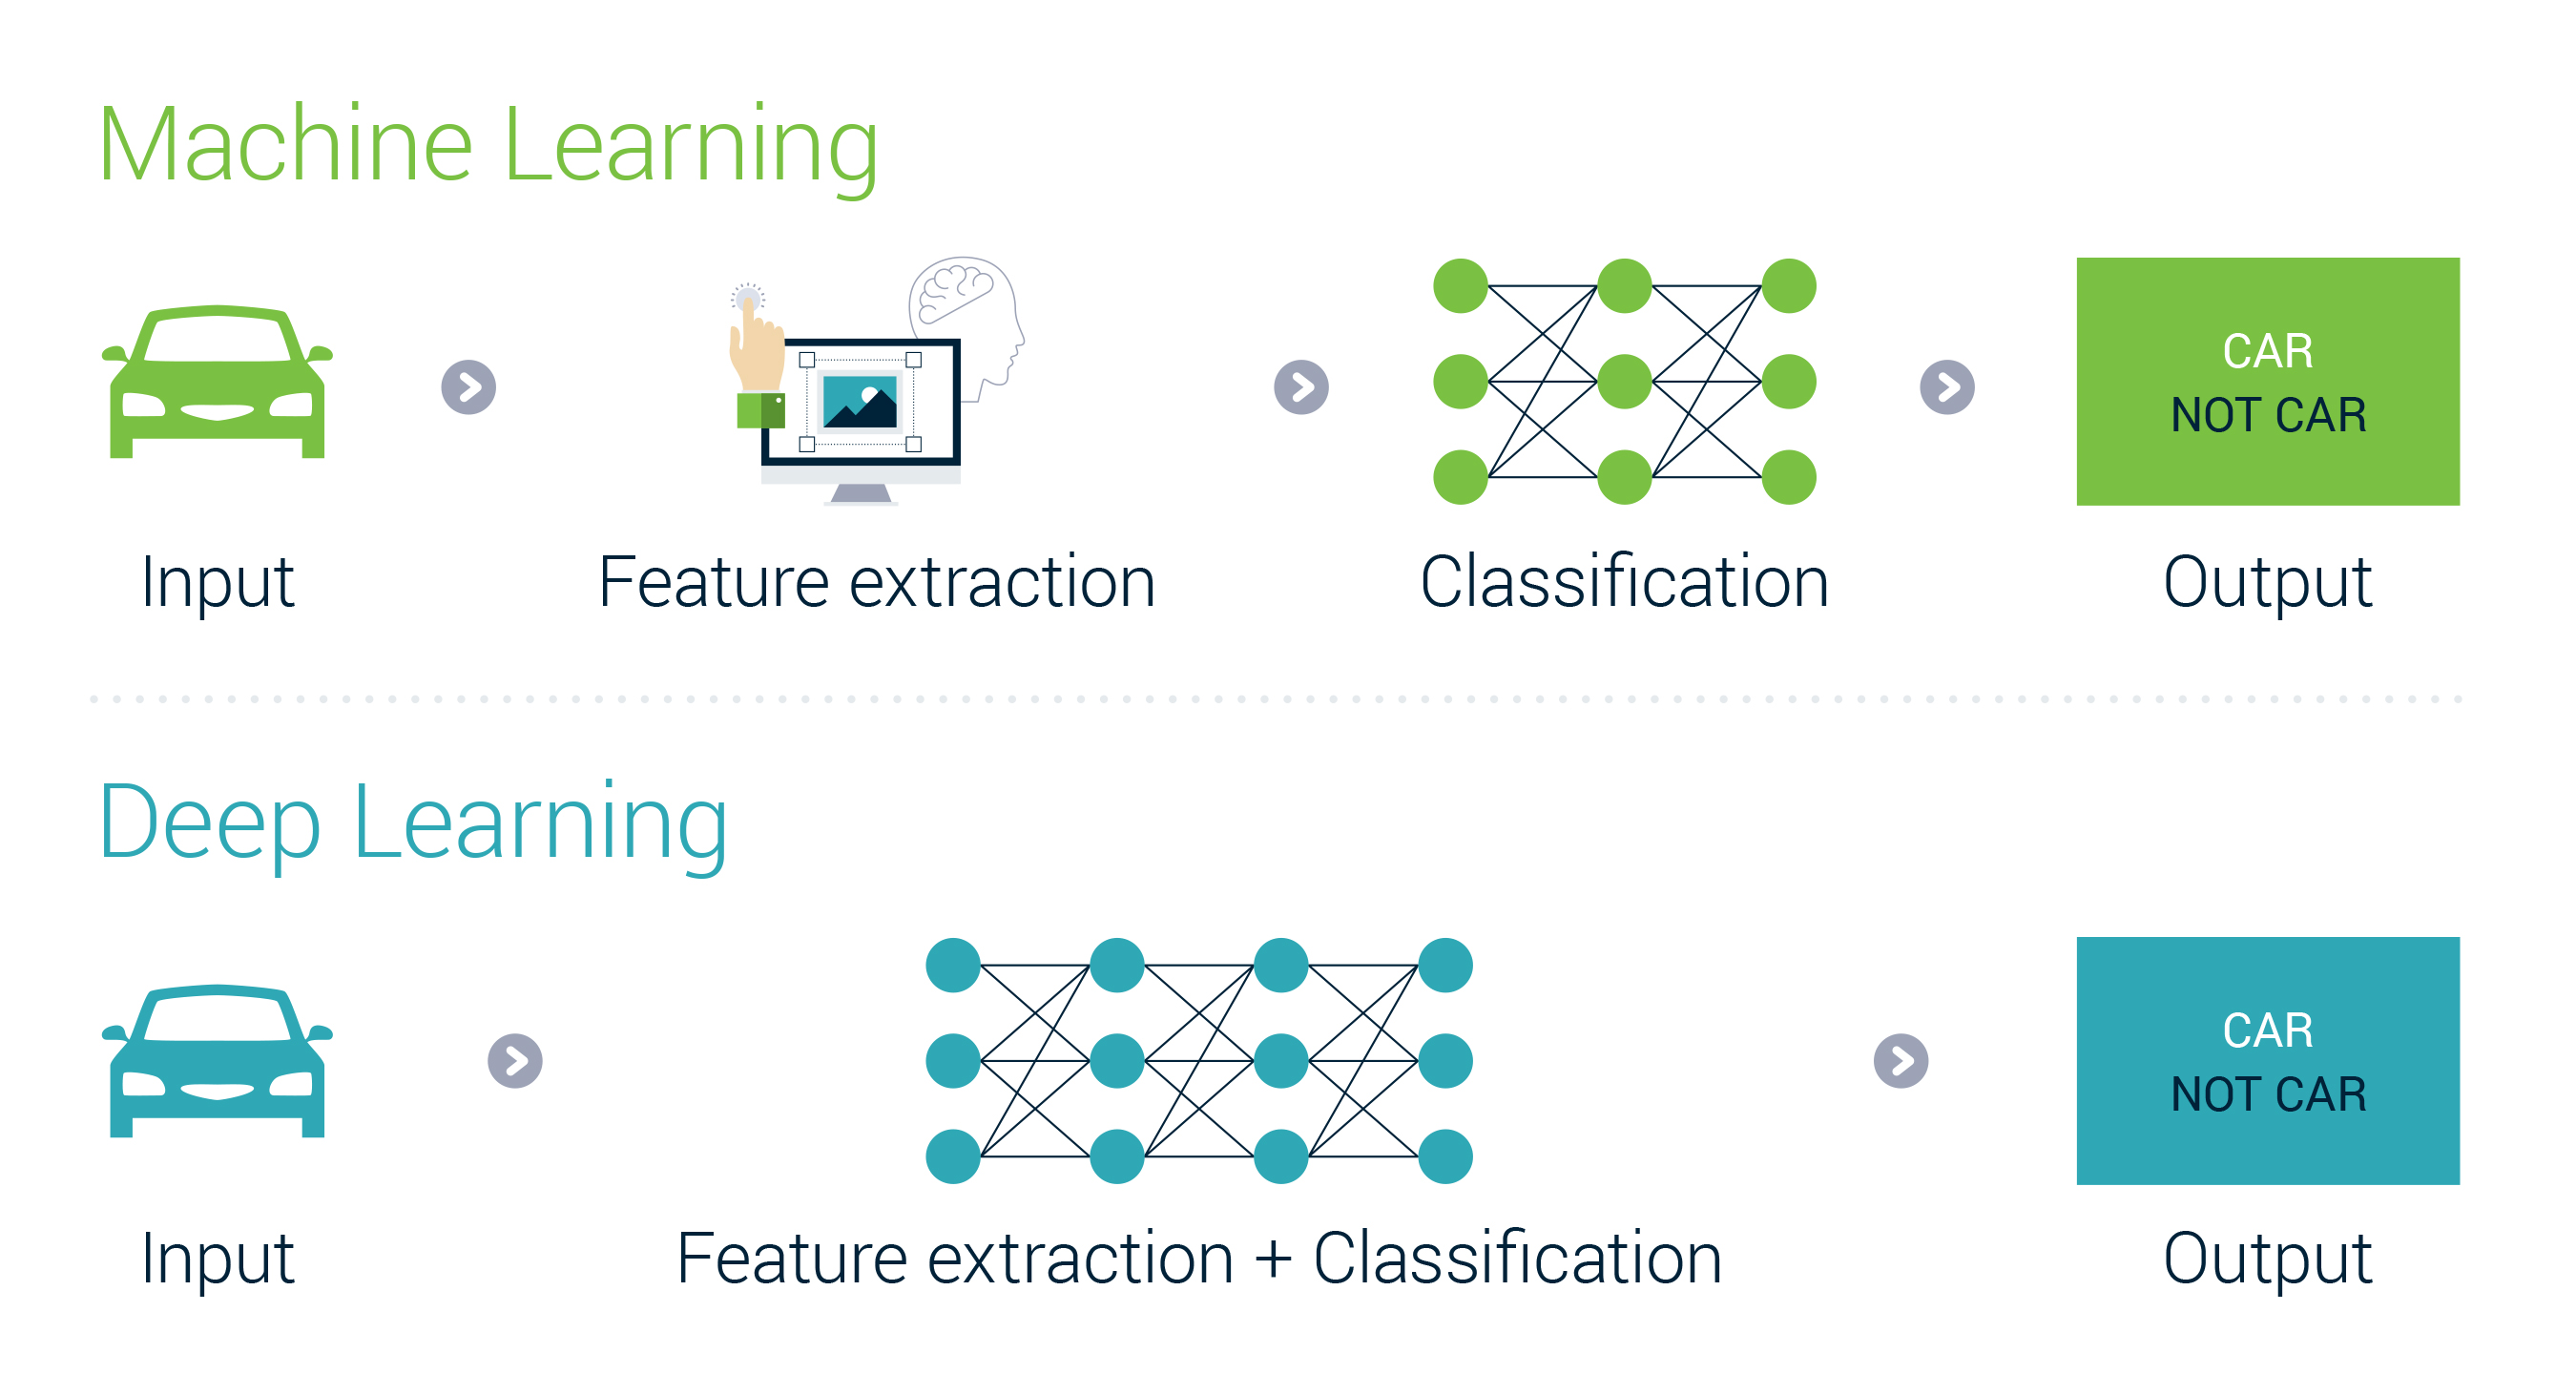
\includegraphics[width=\textwidth]{ml-vs-dl}
  \bicaption[机器学习和深度学习之间的主要区别]{%
    机器学习和深度学习之间的主要区别.
    深度学习拥有\acs*{fx}的能力,而不需要手工设计需要从数据中提取的特征.
  }{%
    The main difference between machine learning and deep learning.
    The feature extraction is an integral part of the deep learning;
    therefore, there is no need to craft the features to be extracted
    from the data.
    \\来源/Credit:
    Jochem Grietens,
    \url{https://verhaert.com/difference-machine-learning-deep-learning/},
    (2019-04-25)
  }
  \label{fig:ml-dl}
\end{figure}

\ac{dl}是\ac{ml}的一个子集,同时后者又是\ac{ai}的一个子集.
\ac{ai}起始于上世纪 50 年代,该领域的开创人之一 John McCarthy 将\ac{ai}定义为
\enquote{制造智能机器的科学和工程} \cite{mcCarthy2007}.
早期的\ac{ai}系统完全基于一整套规则,而这些规则需要明确地由人来定义和实现 (ref???).
\ac{ml}是另一条实现\ac{ai}的途径,通过让机器从数据中学习并调整自身模型,
达到智能化判断或预测的目的.
利用该方法,我们只需要设计机器需要从数据中提取的特征以及相应的学习策略,
而不需要编写每一条具体的规则,有效地减轻了开发\ac{ai}系统的负担 (ref???).
\ac{dl}是\ac{ml}中的一类技术,让机器拥有了\ac{fx}的能力,
进一步降低了开发先进的\ac{ai}系统的难度,极大地拓展了\ac{ai}的应用范围 (ref???).
\autoref{fig:ml-dl} 示意了\ac{ml}和\ac{dl}之间的主要区别.

近十多年以来,\ac{dl}发展迅猛,已经被应用到诸多领域并取得了突破性成果,
详见 \citeay{leCun2015} 综述文.
\ac{dl}方法包括多种\ac{nn} \cite{bengio2009,leCun2015,schmidhuber2015},
比如\ac{dnn}、\ac{cnn}、\ac{rnn}、\ac{ae}.
其中,\ac{ae}能够以无监督 (unsupervised) 的方式从输入数据中发掘有用的特征,
从而学习得到输入数据的一个有效\ac{representation} \cite{bourlard1988}.
因此,\ac{ae}经常被用于数据的\ac{dim-reduction}\cite{hinton2006,wang2014}
和\ac{denoising}\cite{xie2012,lu2013,bengio2013}.
在\ac{ae}的诸多变种中,\ac{cdae}尤其擅长于发掘数据中的抽象、细微的特征 \cite{du2017},
并且已经被成功地用于微弱\ac{gw}信号的\ac{denoising}\cite{shen2017}、
单声道音源的分离\cite{grais2017}、等等.
这些应用说明了 \ac{cdae} 具有从高度时变 (temporal-variable)
的数据中提取微弱信号的出色能力,
因此,值得尝试将 \ac{cdae} 应用于 EoR 信号的分离.
尽管待分离的 EoR 信号的\ac{snr}比上述应用中的情况更低,
但是 EoR 信号、前景辐射以及望远镜的波束效应都是稳定或近似稳定的.

%---------------------------------------------------------------------
\subsection{卷积去噪自编码器}
\label{sec:cdae}

An autoencoder is composed of an encoder and a decoder, which can be
characterised by the functions $f(\cdot)$ and $g(\cdot)$, respectively.
The encoder maps the input $\B{x}$ to an internal code $\B{h}$, i.e.,
$\B{h} = f(\B{x})$, and the decoder tries to reconstruct the desired
signal from the code $\B{h}$, i.e., $\B{r} = g(\B{h})$, where $\B{x}$,
$\B{h}$, and $\B{r}$ are all vectors in this work.
By placing constraints (e.g., dimensionality, sparsity) on the
code $\B{h}$ and training the autoencoder to minimize the
loss $L(\B{r}, \,\B{x})$, which quantifies the difference between the
reconstruction $\B{r}$ and the input $\B{x}$, the autoencoder is expected
to learn the codes that effectively represent the input
(详见 \citeay{goodfellow2016},第 14 章).

In order to make the autoencoder learn a better representation of the input
to achieve better performance, \citet{vincent2008} and \citet{vincent2010} proposed a
novel training strategy based on the denoising criterion:
artificially corrupt the original input $\B{x}$ (e.g., by adding noise),
feed the corrupted input $\B{x}'$ into the autoencoder, and then train it
to reconstruct the original input $\B{x}$ by minimizing the loss
$L(\B{r}, \,\B{x})$.
During this denoising process, the autoencoder is
forced to capture robust features that are critical to accurately
reconstruct the original input.
An autoencoder trained with such a strategy
is called a `denoising autoencoder.'

Classic autoencoders are built with fully connected layers, each neuron of
which is connected with every neuron in the previous layer.
This makes the total number of parameters increase exponentially with the
number of layers.
Meanwhile, the extracted features are forced to be global, which
is suboptimal to represent the input \cite{masci2011}.
On the other hand, convolutional layers, as used in convolutional neural
networks (CNNs),
make use of a set of small filters and share their weights among
all locations in the data \cite{leCun1998}, which allows to
better capture the local features in the data.
Therefore, CNNs generally have two or more orders of magnitude less
parameters than the analogous fully connected neural networks
\cite{grais2017}
and require much less training resources such as memory and time.
Furthermore, multiple convolutional layers can be easily stacked to extract
sophisticated higher-level features by composing the lower-level ones
obtained in previous layers.
This technique guarantees highly expressive CNNs that achieve
outstanding performance in image classification and relevant fields
\cite{krizhevsky2012,simonyan2014,szegedy2015,ma2019}.
By utilising multiple convolutional layers instead of fully connected
layers in a denoising autoencoder, the obtained CDAE gains the powerful
feature extraction capability of CNNs, which helps improve its denoising
performance, and can reconstruct even seriously corrupted signals
\cite{du2017}.
In consequence, the CDAE may be well suited to exploit the complicated
differences between the EoR signal and the foreground emission
for the purpose of separating them accurately.

%---------------------------------------------------------------------
\subsection{网络架构}
\label{sec:architecture}

Both the encoder and decoder parts of the proposed CDAE consist of multiple
convolutional layers.
We do not set a strict boundary between the two parts
because we focus on the feature extraction and denoising capabilities
rather than on the specific formats of the internal codes $\B{h}$.
For the $l$-th convolutional layer that has $m_l$ filters, a set of $m_l$
feature vectors
$\left(\left\{ \B{v}_{i}^{(l)} \right\}; i = 1, 2, \cdots, m_l \right)$
are generated as the output of this layer by convolving the output of the
previous layer
$\left(\left\{ \B{v}_{j}^{(l-1)} \right\}; j = 1, 2, \cdots, m_{l-1} \right)$
with each of the filters, i.e.,
\begin{equation}
  \label{eq:conv}
  \B{v}_{i}^{(l)} = \phi^{(l)} \left( \sum_{j=1}^{m_{l-1}}
    \B{v}_{j}^{(l-1)} * W_i^{(l)} + b_i^{(l)} \right),
    \quad i = 1, 2, \cdots, m_{l},
\end{equation}
where
$W_i^{(l)}$ and $b_i^{(l)}$ are the weights and bias of this filter
in the $l$-th layer, $\phi^{(l)}(\cdot)$ is the layer's activation
function, and `$*$' denotes the convolution operation.

Following the common practices \cite{geron2017,suganuma2018},
we adopt filters of size 3 in all layers and use the exponential linear
unit (ELU) \cite{clevert2016} as the activation function
$\phi^{(l)}(\cdot)$ for all layers except the last layer, which uses
the hyperbolic tangent function (i.e., tanh;
see also \autoref{sec:preprocessing}).
In addition, the batch normalisation technique is applied to all layers
except for the last layer to improve the training process as well as to act
as a regularizer to prevent over-fitting \cite{ioffe2015}.

To determine the number of convolutional layers and the number of filters
in each layer, we have tested multiple CDAE architectures, each containing
a different number of layers and filters.
After evaluating their performances (see also \autoref{sec:cdae-results}),
the simplest one with sufficiently good performance is selected,
which consists of a 4-layer encoder with $(32,64,64,32)$ filters and
a 5-layer decoder with $(32,64,64,32,1)$ filters, as illustrated in
\autoref{fig:cdae-network}.
We note that the pooling and upsampling layers are not used in the CDAE
because they have very little impact on the performance according to our
tests
(另可参见 \citeay{springenberg2015}).

\begin{figure}[htp]
  \centering
  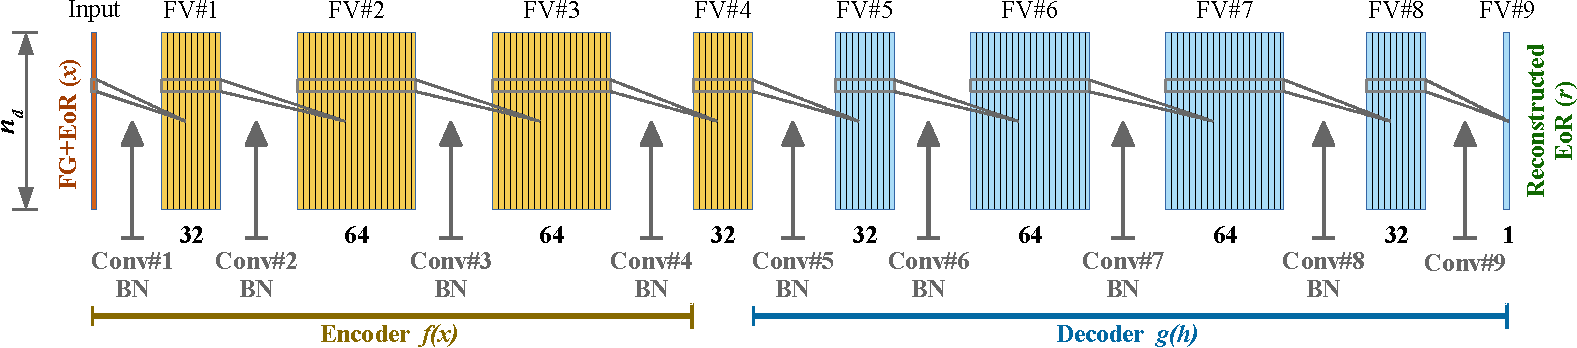
\includegraphics[width=\textwidth]{cdae-network-crop}
  \bicaption[CDAE 网络架构示意图]{%
    TODO...
  }{%
    The architecture of the proposed CDAE that consists of a 4-layer
    encoder and a 5-layer decoder.
    The orange and blue boxes represent the feature vectors (FV) generated
    by the encoder and decoder layers, respectively.
    The numbers marked below the boxes are the number of filters in the
    corresponding convolutional layers.
    The batch normalization (BN) technique is applied to all layers except
    for the last layer.
  }
  \label{fig:cdae-network}
\end{figure}

%---------------------------------------------------------------------
\subsection{训练和评估方法}
\label{sec:train-eval}

At the beginning, the parameters of the CDAE (i.e., the weights and biases
of filters in all layers) are initialised randomly using the He uniform
initialiser \cite{he2015}.
In order to obtain an effective CDAE by
training these parameters, the
following three datasets are required \cite{ripley1996}:
(1) training set ($S_{\R{tr}}$) that is used to fit the parameters;
(2) validation set ($S_{\R{val}}$)
that is used not only to validate whether or not the training
process runs well (e.g., no over-fitting), but also to
help determine the hyperparameters (e.g., the number of layers and filters;
\autoref{sec:architecture});
(3) test set ($S_{\R{test}}$) that is solely used to evaluate the
performance of the trained CDAE.
Each dataset is a collection of many data points of
($\B{x}, \B{x}_{\R{eor}}$),
where $\B{x} = \B{x}_{\R{eor}} + \B{x}_{\R{fg}}$ is the total emission of
one sky pixel, and $\B{x}_{\R{eor}}$ is the corresponding EoR signal.

During each training epoch, the total emission $\B{x}^{(i)}$ is fed into
the CDAE and goes through all the convolutional layers (\autoref{eq:conv}),
outputting the reconstructed EoR signal $\B{r}^{(i)}_{\R{eor}}$.
The difference between the reconstructed EoR signal $\B{r}^{(i)}_{\R{eor}}$
and the input EoR signal $\B{x}^{(i)}_{\R{eor}}$ is the loss $L$ and can be
quantified with the mean squared error (MSE), i.e.,
\begin{equation}
  \label{eq:loss}
  L = \frac{1}{N_{\R{tr}}} \sum_{i=1}^{N_{\R{tr}}}
    \left[ \B{r}_{\R{eor}}^{(i)} - \B{x}_{\R{eor}}^{(i)} \right]^T
    \left[ \B{r}_{\R{eor}}^{(i)} - \B{x}_{\R{eor}}^{(i)} \right],
\end{equation}
where $N_{\R{tr}}$ is the number of data points in the training set
$S_{\R{tr}}$.
By applying the back-propagation method
\cite{rumelhart1986,leCun1998bp},
the parameters are updated to reduce the loss $L$, so as to
improve the quality of the reconstructed EoR signal.
As the training goes for more epochs, the initially randomised CDAE is
gradually shaped into a network
that learns a better representation of the input and can
reconstruct the EoR signal more accurately.

To evaluate the performance of the trained CDAE,
the Pearson's correlation coefficient
\cite{harker2009,chapman2013}
is adopted to measure the similarity between the reconstructed and input
EoR signals:
\begin{equation}
  \label{eq:corrcoef}
  \rho(\B{r}_{\R{eor}}, \B{x}_{\R{eor}})
      = \frac{\sum_{j=1}^{n}(r_{\R{eor},j} - \bar{r}_{\R{eor}})
      (x_{\R{eor},j} - \bar{x}_{\R{eor}})}{
        \sqrt{\sum_{j=1}^{n}(r_{\R{eor},j} - \bar{r}_{\R{eor}})^2
          \sum_{j=1}^{n}(x_{\R{eor},j} - \bar{x}_{\R{eor}})^2}
    },
\end{equation}
where
$\bar{r}_{\R{eor}}$ and $\bar{x}_{\R{eor}}$ represent the mean
values of $\B{r}_{\R{eor}}$ and $\B{x}_{\R{eor}}$, respectively, and $n$
is the length of the signals.
The closer to one the correlation coefficient
$\rho(\B{r}_{\R{eor}}, \B{x}_{\R{eor}})$ is,
the better the achieved performance.


%=====================================================================
\section{新算法的演示}

experiment, demonstration

%---------------------------------------------------------------------
\subsection{数据集}
\label{sec:cdae-dataset}

We carry out end-to-end simulations to generate the SKA images to
train the proposed CDAE and evaluate its performance.
A representative frequency band, namely \SIrange{154}{162}{\MHz}, is chosen
as an example \cite{datta2010} and is divided into $n_f = 101$
channels with a resolution of \SI{80}{\kHz}.
At each frequency channel, the sky maps of the foreground emission and the
EoR signal are simulated within an area of \SI{10 x 10}{\degree} and are
pixelized into \num{1800 x 1800} with a pixel size of \SI{20}{\arcsecond}.

\begin{figure}[htp]
  \centering
  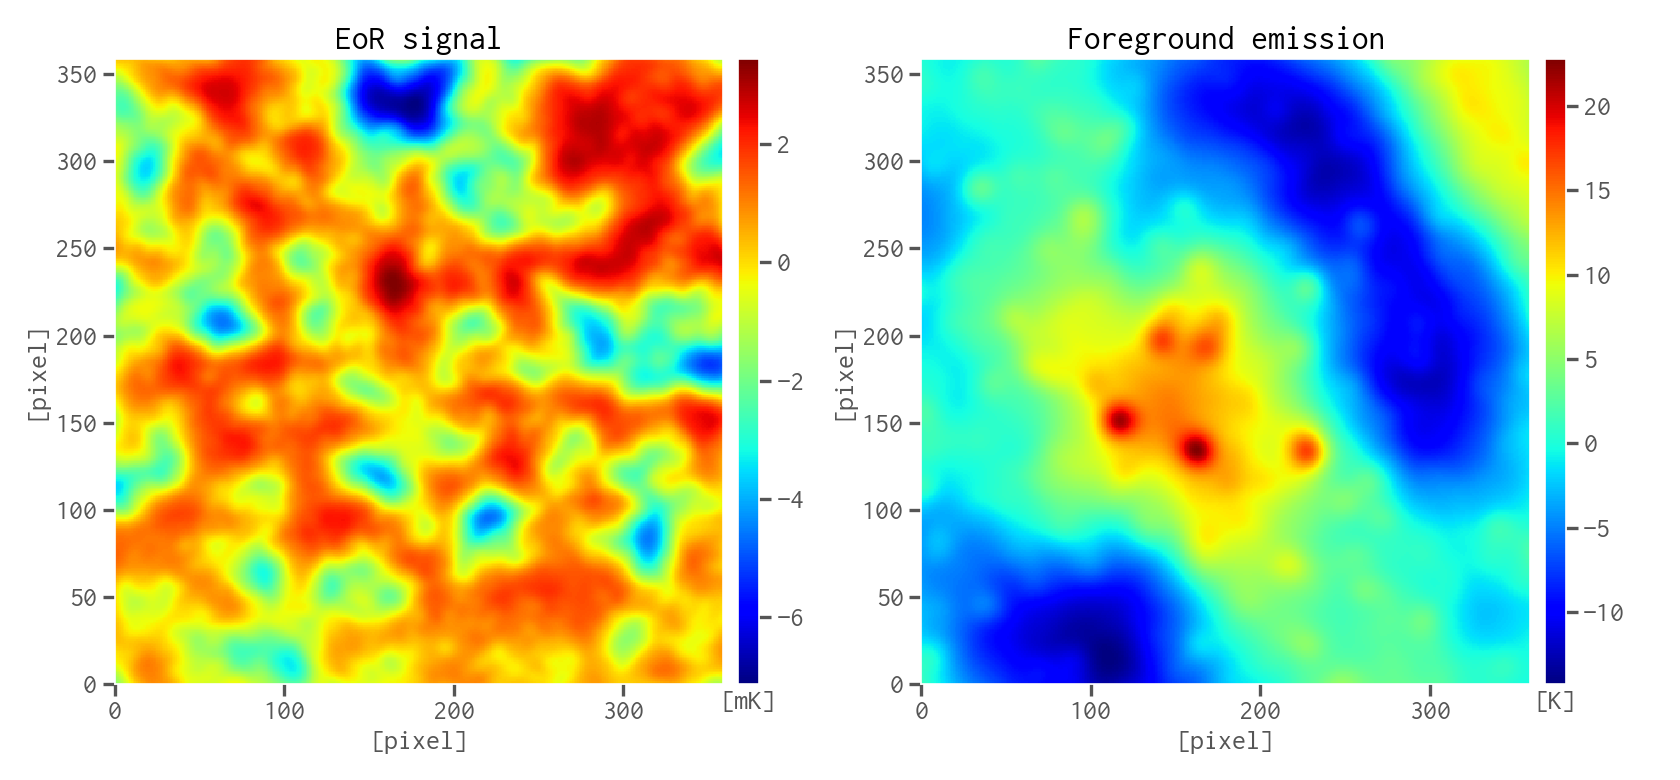
\includegraphics[width=\textwidth]{eor-fg-obsimg-158}
  \bicaption[EoR 信号和前景在 \SI{158}{\MHz} 的模拟图像]{%
    TODO...
  }{%
    Simulated images of the EoR signal (left panel) and the foreground
    emission (right panel) at \SI{158}{\MHz}.
    Both images have sizes of \num{360 x 360} and cover sky areas of
    \SI{2 x 2}{\degree}.
    The blobs in the right panel show the bright point sources and radio
    haloes.
  }
  \label{fig:eor-fg-obsimg}
\end{figure}

Based on our previous work \cite{wang2010}, we simulate the foreground
emission by taking into account the contributions from the Galactic
synchrotron and free-free radiations, extragalactic point sources, and
radio haloes.
The Galactic synchrotron radiation is simulated by extrapolating the Haslam
\SI{408}{\MHz} map with a power-law spectrum, the index of which is given
by the synchrotron spectral index map \cite{giardino2002} to account for
its variation with sky positions.
The reprocessed Haslam \SI{408}{\MHz} map\footnote{%
  The reprocessed Haslam \SI{408}{\MHz} map:
  \url{http://www.jb.man.ac.uk/research/cosmos/haslam_map/}}
\cite{remazeilles2015}, which has significantly better instrument
calibration and more accurate extragalactic source subtraction,
is used as the template to obtain enhanced simulation results over
\citet{wang2010}.
By employing the tight relation between the Hα and free-free
emissions (参见 \citeay{dickinson2003} 及其所引文献),
the Galactic free-free radiation can be derived from the Hα survey map
\cite{finkbeiner2003}.
Since the Galactic diffuse emissions vary remarkably across the sky, we
simulate them at a central position of (R.A., Dec.\@) = (\SI{0}{\degree},
\SI{-27}{\degree}), which has a high galactic latitude
($b = \SI{-78.5}{\degree}$) and is an appropriate choice for the simulation
of SKA images \cite{beardsley2016}.
We account for the following 5 types of extragalactic point sources:
(1) star-forming and starburst galaxies, (2) radio-quiet active galactic
nuclei (AGNs), (3) Fanaroff-Riley type I and type II AGNs, (4) GHz-peaked
spectrum AGNs, and (5) compact steep spectrum AGNs.
The former three types of sources are simulated by utilising the data
published by \citet{wilman2008} and the latter two types are simulated by
employing their corresponding luminosity functions and spectral models.
Similar to the real-time peeling of the brightest point sources in
practical data analysis pipelines \cite{mitchell2008,intema2009},
we assume that sources with a \SI{158}{\MHz} flux density
$S_{158} > \SI{10}{\mJy}$ have been removed \cite{liu2009ps}.
The radio haloes are simulated by generating a sample of galaxy clusters
with the Press-Schechter formalism \cite{press1974} and then applying
multiple scaling relations (e.g., between cluster mass and X-ray
temperature, between X-ray temperature and radio power) to derive their
radio emissions.

In regard to the simulation of the EoR signal, we take advantage of the
2016 data release from the
\textit{Evolution Of 21\,cm Structure} project\footnote{%
  Evolution Of 21\,cm Structure:
  \url{http://homepage.sns.it/mesinger/EOS.html}}
\cite{mesinger2016} and extract the image slices at corresponding
redshifts (i.e., frequencies) from the light-cone cube of the recommended
`faint galaxies' case.
The extracted image slices are then re-scaled to match the sky coverage and
pixel size of the foreground maps.

To incorporate the realistic frequency-dependent beam effects into the
simulated sky maps, we further adopt the latest SKA1-Low layout
configuration\footnote{\raggedright%
  SKA1-Low layout:
  \url{https://astronomers.skatelescope.org/wp-content/uploads/2016/09/SKA-TEL-SKO-0000422_02_SKA1_LowConfigurationCoordinates-1.pdf}}
to simulate instrument observations.
The SKA1-Low interferometer is composed of 512 stations, each of which
contains 256 antennas randomly distributed inside a circle of
\SI{35}{\meter} in diameter.
The 512 stations are divided into two parts:
(1) 224 stations are randomly distributed within the `core' region of
\SI{1000}{\meter} in diameter;
(2) the remaining stations are placed on 3 spiral arms extending up to a
radius of about \SI{35}{\kilo\meter}.
For each sky map, we employ the \textsc{OSKAR}\footnote{%
  OSKAR: \url{https://github.com/OxfordSKA/OSKAR} (version 2.7.0)}
simulator \cite{mort2010} to perform 6-hour synthesis imaging
to obtain the visibility data, from which the `observed'
image is created by the \textsc{WSClean}\footnote{%
  WSClean: \url{https://sourceforge.net/p/wsclean} (version 2.5)}
imager \cite{offringa2014}.
In order to emphasize the faint and relatively diffuse EoR signal, the
natural weighting and baselines of \numrange{30}{1000} wavelengths are
utilised in the imaging process.
Finally, the created images are cropped to keep only the central
\SI{2 x 2}{\degree} regions (i.e., \num{360 x 360} pixels) for the
purpose of the best quality.
Therefore, we obtain a pair of image cubes of size
\num{360 x 360 x 101} for the EoR signal $\left( C_{\R{eor}}^{(1)} \right)$
and the foreground emission $\left( C_{\R{fg}}^{(1)} \right)$, respectively
(see \autoref{fig:eor-fg-obsimg} for the simulated images at the
central frequency of \SI{158}{\MHz}).
To better illustrate the impacts of beam effects on the foreground spectra,
we take one random sky pixel as an example and show the foreground
spectra with and without the beam effects in \autoref{fig:cdae-simdata}, where
the corresponding differential spectra (i.e., differences between every
two adjacent frequency channels) and the EoR signal spectrum are also
plotted.
Compared to the ideal sky foreground (the top panel), the spectral
smoothness of the `observed' foreground (the middle panel) is seriously
damaged by the rapid fluctuations resulted from the beam effects.
Although such fluctuations exhibit somewhat similar spectral scales
($< \SI{1}{\MHz}$) as the EoR signal (the bottom panel), they are
still sufficiently different, which can be exploited by the CDAE to achieve
an effective separation.
We note that the `observed' foreground has an amplitude of about two orders
of magnitude smaller than the ideal foreground, the major reason for which
is that interferometers are only sensitive to the spatial fluctuations of
the emission \cite{braun1985}.

\begin{figure}[htp]
  \centering
  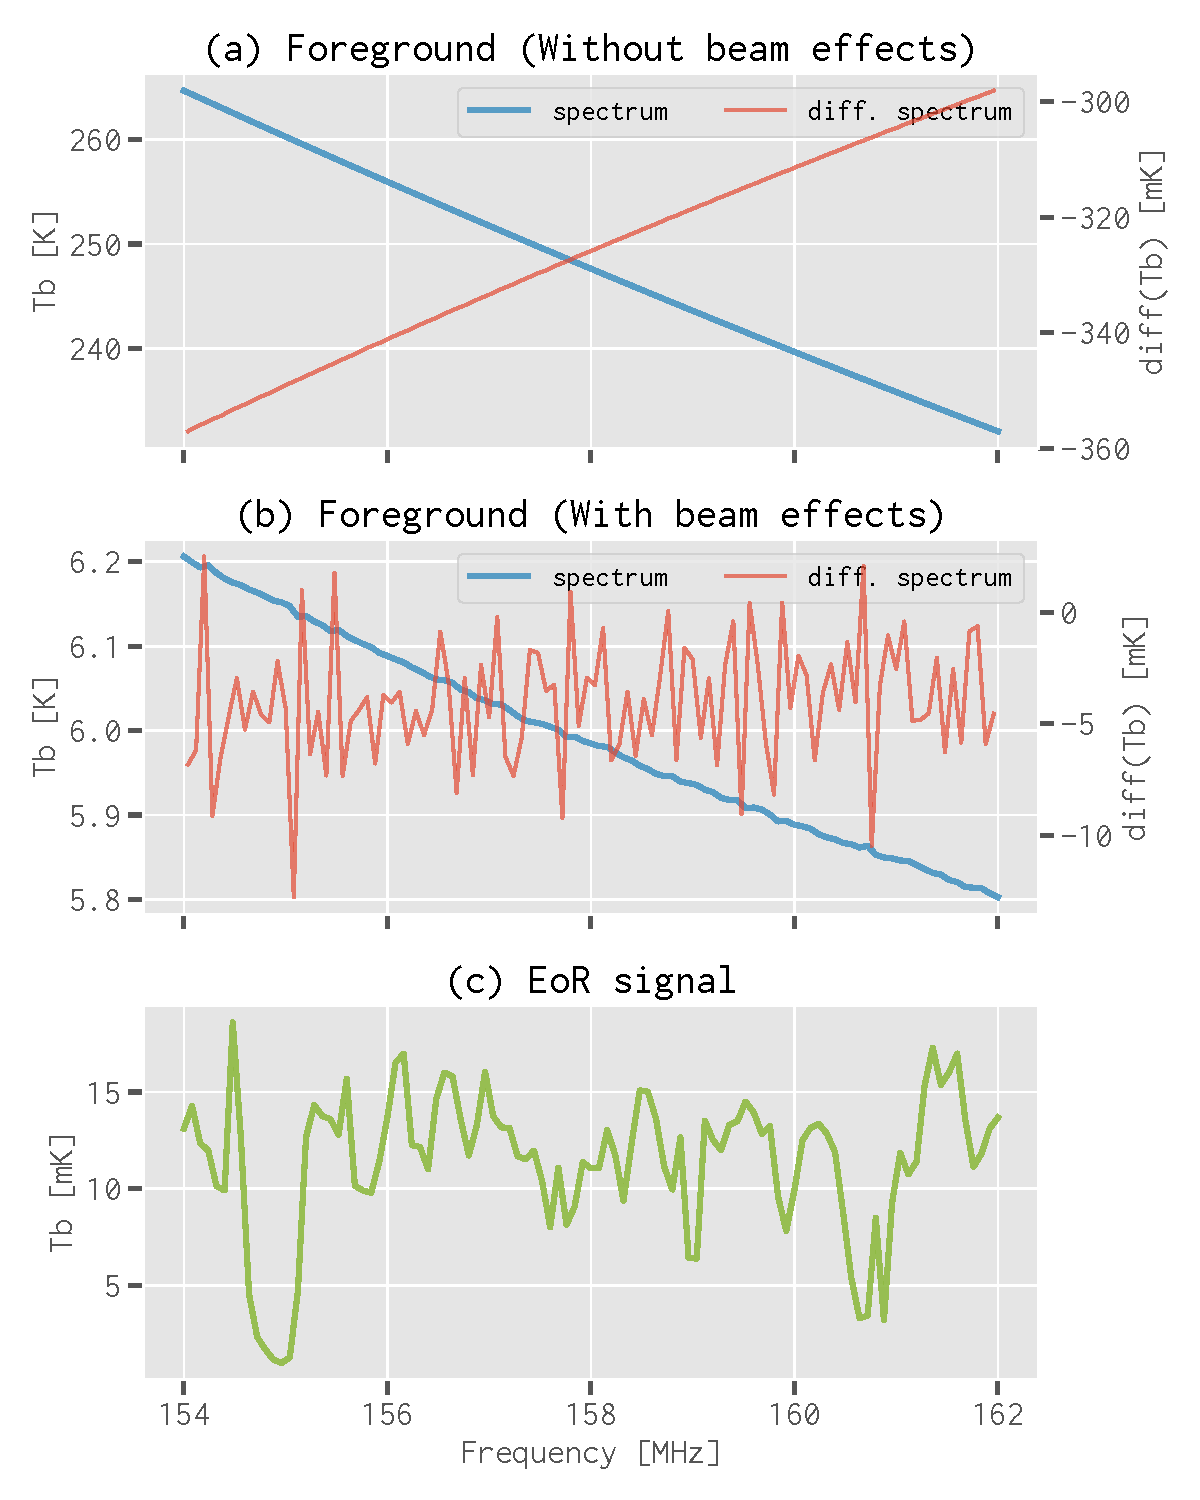
\includegraphics[width=0.9\textwidth]{cdae-simdata-example}
  \bicaption[前景辐射和 EoR 信号的频谱示例]{%
    TODO...
  }{%
    Example spectra of the foreground emission and the EoR signal for one
    random sky pixel.
    \textbf{Top}: the ideal (i.e., without beam effects) foreground
    spectrum (the blue line) and the corresponding differential spectrum
    (the red line).
    \textbf{Middle}: the `observed' (i.e., with beam effects) foreground
    spectrum (the blue line) and the corresponding differential spectrum
    (the red line).
    \textbf{Bottom}: the EoR signal spectrum (the green line).
  }
  \label{fig:cdae-simdata}
\end{figure}

Considering that the training and evaluation of the CDAE require three
datasets (i.e., training, validation, and test; \autoref{sec:train-eval}),
if there are only one pair of image cubes, the test set $S_{\R{test}}$
could only contain a small fraction of all the pixels that are randomly
distributed on the sky, from which it is impossible to obtain a complete
image of the reconstructed EoR signal.
Consequently, it is beneficial to simulate another pair of image cubes
that are solely used as the test set.
To this end, we simulate the Galactic diffuse radiations at a central
coordinate of (R.A., Dec.\@) = (\SI{3}{\degree}, \SI{-27}{\degree}), i.e.,
\SI{3}{\degree} away from the first pair of image cubes, which is
sufficient because the finally cropped image cubes only cover a sky area of
\SI{2 x 2}{\degree}.
Since extragalactic point sources, radio haloes, and the EoR signal are
mostly isotropic, we shift their sky maps simulated above by
\SI{3}{\degree} to generate the new sky maps.
Following the same procedures to simulate instrument observations, we
obtain the second pair of image cubes
$\left( C_{\R{eor}}^{(2)}, C_{\R{fg}}^{(2)} \right)$.

We note that the simulations do not include thermal noise because the
proposed method is designed to create tomographic EoR images from very deep
observations that have a sufficiently low noise level.
The SKA1-Low is planned to observe each of the target fields for
about \SI{1000}{\hour}, reaching an unprecedented image noise level of
$\,\lesssim \SI{1}{\mK}$ that allows to directly image the reionization
structures
\cite{mellema2013,mellema2015,koopmans2015}.

%---------------------------------------------------------------------
\subsection{数据预处理}
\label{sec:preprocessing}

The dataset $S = \{(\B{x}, \,\B{x}_{\R{eor}})\}$ for the CDAE is derived
from the simulated image cubes $C_{\R{eor}}$ and $C_{\R{fg}}$, each data
point $(\B{x} = \B{x}_{\R{eor}} + \B{x}_{\R{fg}}, \,\B{x}_{\R{eor}})$
representing the total emission and the EoR signal of one sky pixel,
respectively.
The dataset thus has $N_S = \num{360x360 x 2} = \num{259200}$
data points in total.

For the input data $X = \{\B{x}\}$, we propose to apply the
Fourier Transform (FT) along the frequency dimension,
which makes the EoR signal more distinguishable from the
foreground emission and thus easier to be learned by the CDAE
(a comparison with the results derived without applying the FT is
presented in \autoref{sec:why-ft}).
The Blackman--Nuttall window function is applied to suppress the
FT side-lobes caused by the sharp discontinuities at both ends
of the finite frequency band \cite{chapman2016}.
It is sufficient to keep only half the Fourier coefficients because
$\B{x}$ is real, thus $\B{x}$ of length $n_f = 101$ is transformed to
be 51 complex Fourier coefficients.
The $n_{\R{ex}}$ coefficients of the lowest Fourier frequencies are
excised since they are mostly contributed by the spectral-smooth
foreground emission.
We adopt $n_{\R{ex}} = 6$ to achieve a balance between the
foreground emission suppression and the EoR signal loss.
The real and imaginary parts of the remaining 45 complex coefficients
are then concatenated into a new real vector of length $n_d = 90$,
since the CDAE requires real data.
Finally, the data are zero-centred and normalised to have unit variance.

The preprocessing steps for the input EoR signal
$X_{\R{eor}} = \{\B{x}_{\R{eor}}\}$
are basically the same except for minor adjustments.
After applying the FT, excising the $n_{\R{ex}}$ lowest Fourier
components, and concatenating the real and imaginary parts,
the data elements that have a value less than the 1$^{\R{st}}$
percentile or greater than the 99$^{\R{th}}$ percentile are truncated,
in order to prevent the possible outliers from hindering the training of
the CDAE.
Finally, the value range of the data is scaled to $[-1, 1]$ by
dividing by the maximum absolute value,
which allows to use the `tanh' activation function whose value range
is also $[-1, 1]$ in the output layer of the proposed CDAE
(\autoref{sec:architecture}).

%---------------------------------------------------------------------
\subsection{训练和结果}
\label{sec:cdae-results}

The preprocessed data of the first cube pair
$\left( C_{\R{eor}}^{(1)}, C_{\R{fg}}^{(1)} \right)$
are randomly partitioned into the training set ($S_{\R{tr}}$; corresponding
to 80 per cent of the pixels, or \num{103680} data points) and the
validation set ($S_{\R{val}}$; 20 per cent, or \num{25920} data points).
The preprocessed data of the second cube pair
$\left( C_{\R{eor}}^{(2)}, C_{\R{fg}}^{(2)} \right)$
are solely used as the test set ($S_{\R{test}}$; \num{129600} data points).
The use of the whole image cubes as the test set enables us to create
complete images of the reconstructed EoR signal.

We implement the proposed CDAE using the
\href{https://keras.io}{\texttt{Keras}}\footnote{%
  Keras: \url{https://keras.io} (v2.2.4)}
framework \cite{keras} with the
\href{https://www.tensorflow.org}{\texttt{TensorFlow}}\footnote{%
  TensorFlow: \url{https://www.tensorflow.org} (v1.12.0)}
back end \cite{tensorflow},
which is accelerated by the
\href{https://developer.nvidia.com/cuda-zone}{\texttt{CUDA}}\footnote{%
  CUDA: \url{https://developer.nvidia.com/cuda-zone} (v9.1.85)}
toolkit.
We adopt a small initial learning rate ($\alpha = \num{e-5}$) and use the
Adam optimisation method \cite{kingma2015}.
The CDAE is trained on the training set ($S_{\R{tr}}$) with a batch size of
100 until the training loss converges, which takes about 50 epochs.

\begin{figure}[htp]
  \centering
  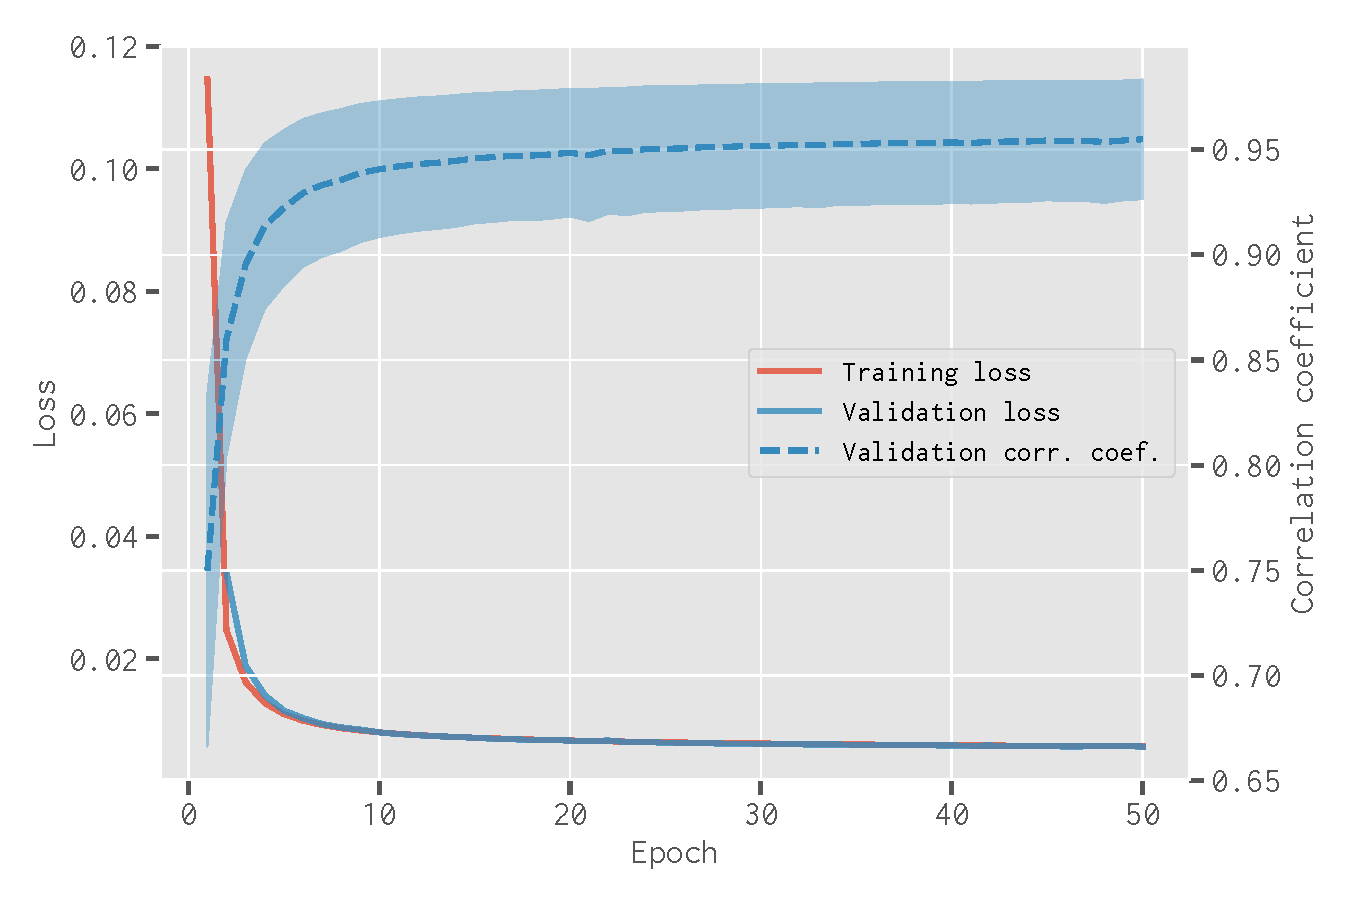
\includegraphics[width=\textwidth]{cdae-train}
  \bicaption[训练 CDAE 的过程和结果]{%
    TODO...
  }{%
    The training loss (solid red line), validation loss (solid blue
    line), and correlation coefficient ($\rho$; dashed blue
    line with the shaded region representing its standard deviation)
    calculated on the validation set $S_{\R{val}}$ along the training of
    the CDAE.
  }
  \label{fig:cdae-train}
\end{figure}

\begin{figure}[htp]
  \centering
  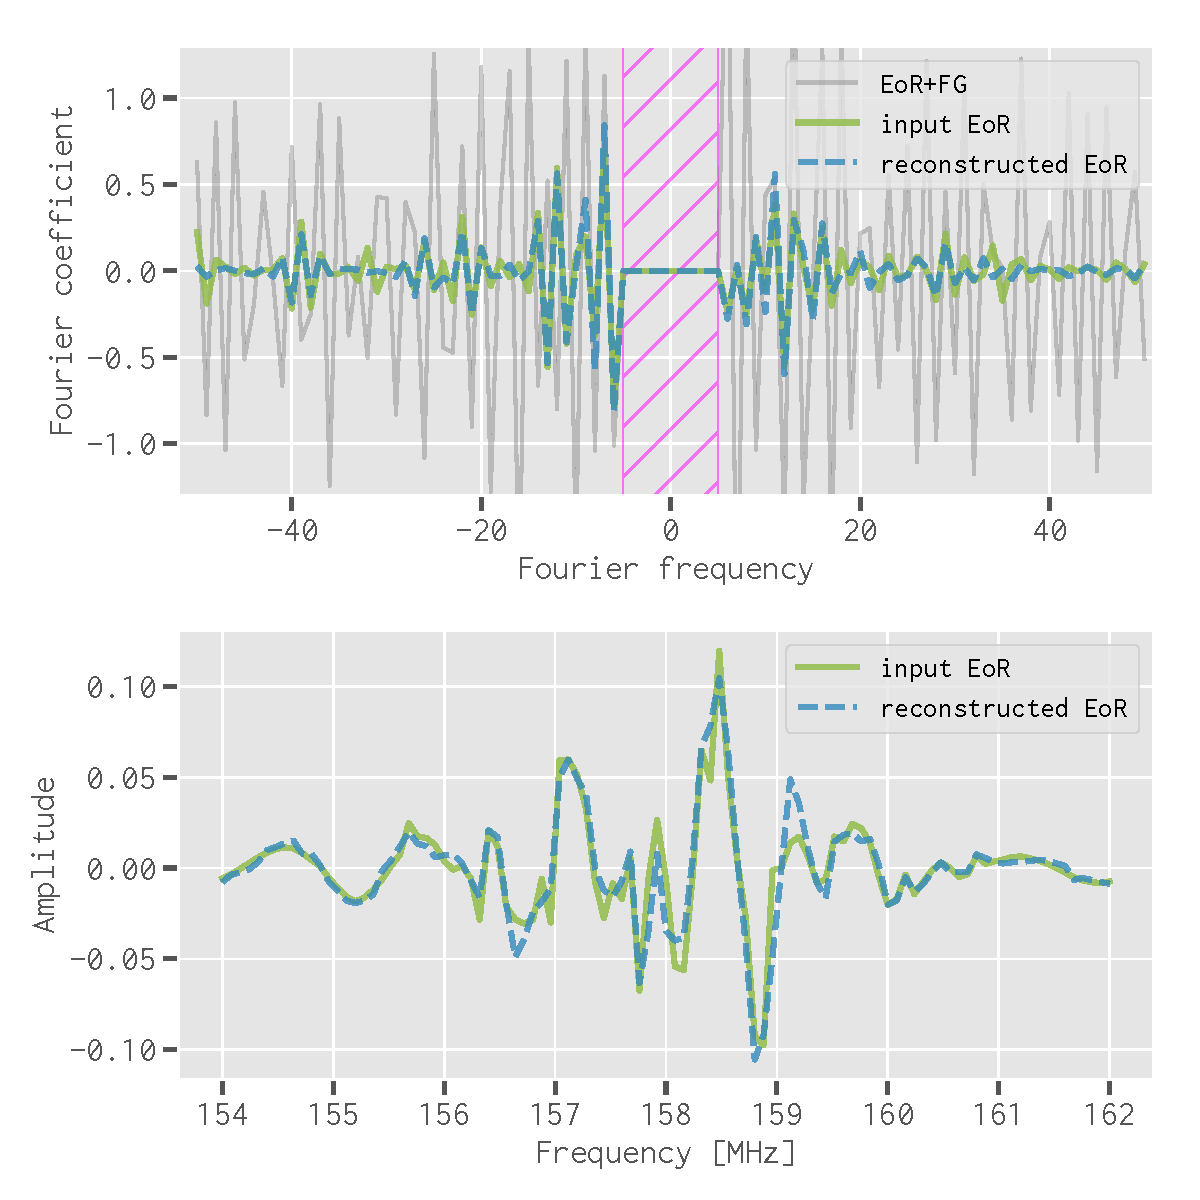
\includegraphics[width=\textwidth]{cdae-eor-pix}
  \bicaption[CDAE 重建的 EoR 信号的示例]{%
    TODO...
  }{%
    An example of the EoR signal reconstructed by the trained CDAE for
    one pixel in $S_{\R{test}}$.
    \textbf{(top)} The input EoR signal $\B{x}_{\R{eor}}$ (solid
    green line) and the reconstructed EoR signal $\B{r}_{\R{eor}}$
    (dashed blue line) in the Fourier domain.
    The correlation coefficient between the input and
    reconstructed EoR signals is $\rho = 0.931$.
    The gray line represents the input total emission
    $\B{x} = \B{x}_{\R{fg}} + \B{x}_{\R{eor}}$.
    The magenta hatched region marks the excised Fourier coefficients
    in data preprocessing.
    \textbf{(bottom)} The input EoR signal $\B{x}_{\R{eor}}$ (solid
    green line) and the reconstructed EoR signal $\B{r}_{\R{eor}}$
    (dashed blue line) transformed back to the observing frequency
    domain.
  }
  \label{fig:cdae-eor-pix}
\end{figure}

The training and validation losses together with the evaluation index
(i.e., the correlation coefficient $\rho$) calculated on the validation set
$S_{\R{val}}$ during the training phase are shown in \autoref{fig:cdae-train}.
The steadily decreasing losses and increasing correlation coefficient
suggest that the CDAE is well trained without over-fitting.
After training, the evaluation with the test set $S_{\R{test}}$ yields a
high correlation coefficient of $\bar{\rho}_{\R{cdae}} = \num{0.929 +- 0.045}$
between the reconstructed and input EoR signals.
This result demonstrates
that the trained CDAE achieves excellent performance in reconstructing the
EoR signal.
As an example, \autoref{fig:cdae-eor-pix} illustrates the reconstructed EoR
signal ($\rho = 0.931$) for one pixel in $S_{\R{test}}$.

\begin{figure}[htp]
  \centering
  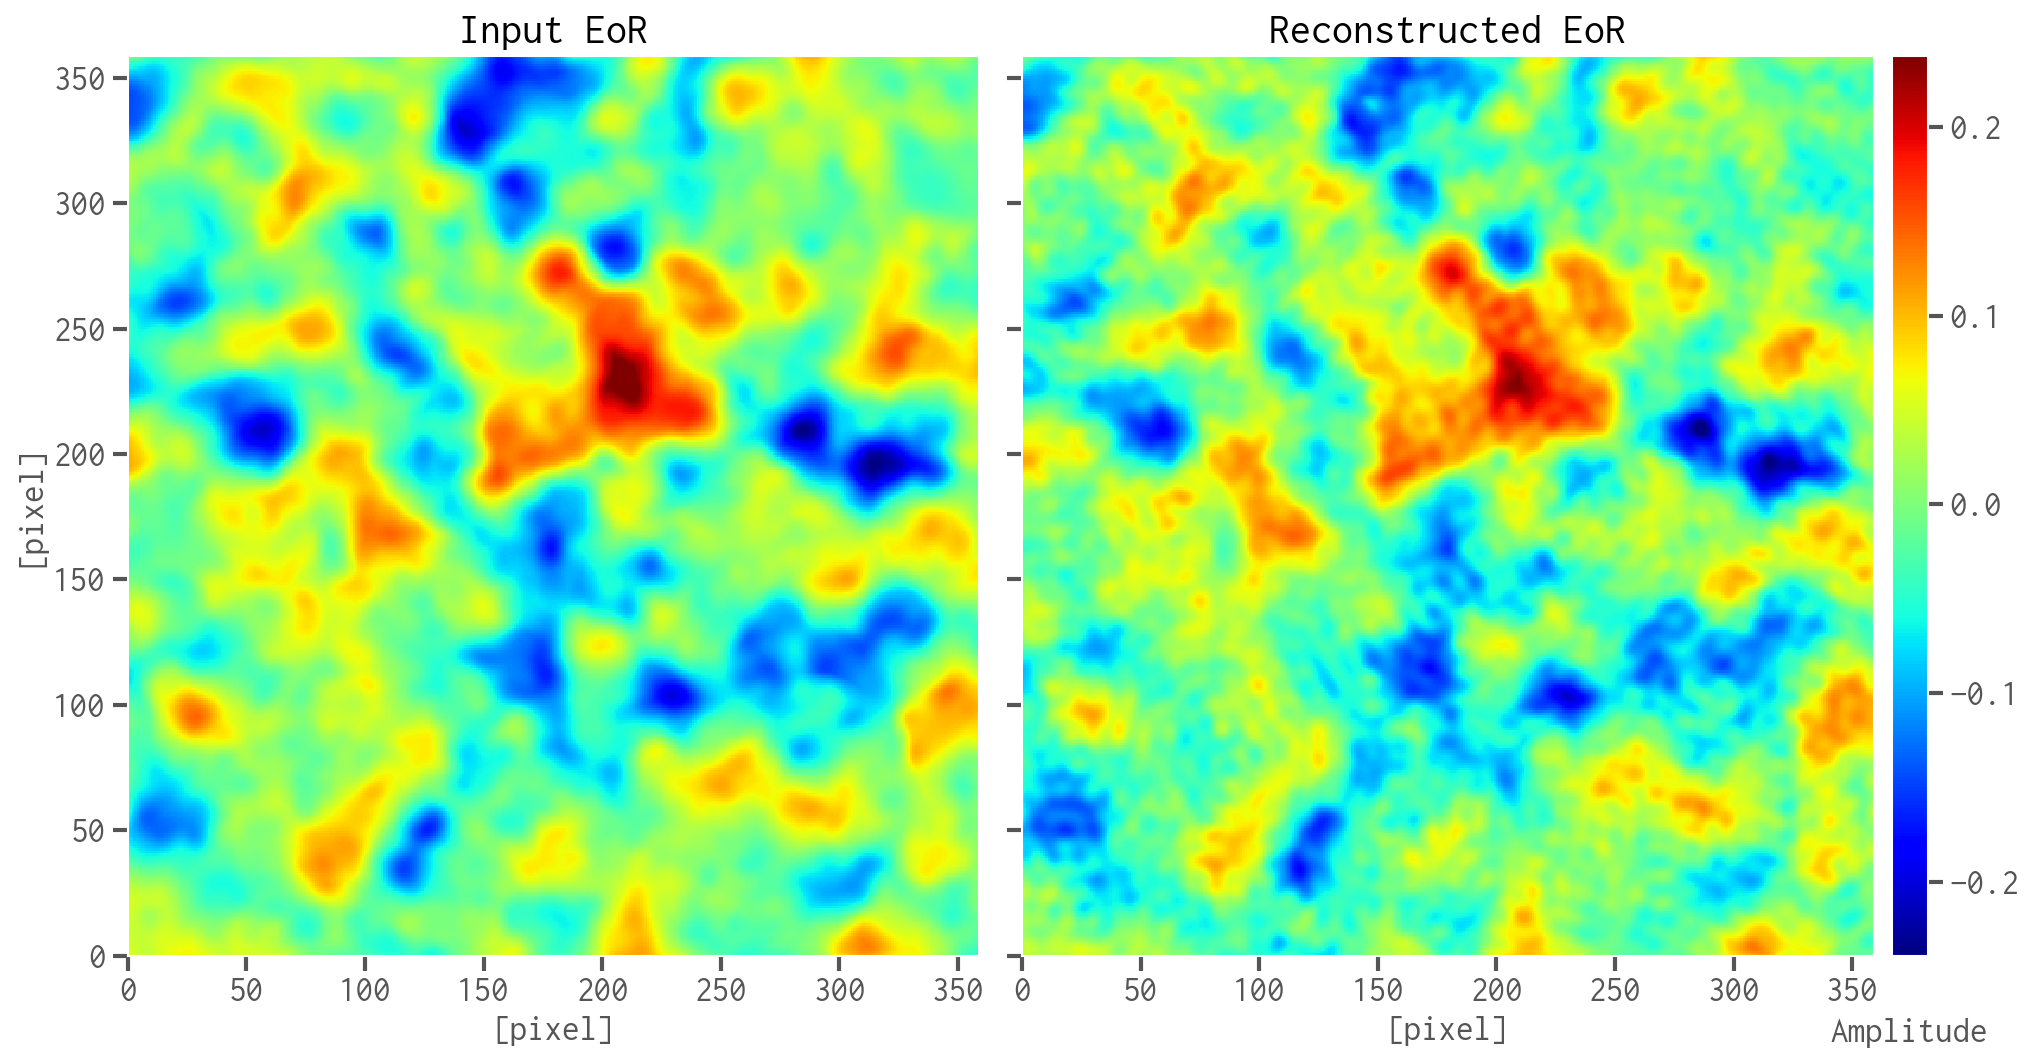
\includegraphics[width=\textwidth]{cdae-eor-img-comp}
  \bicaption[输入的 EoR 图像和 CDAE 重建的 EoR 图像的对比]{%
    TODO...
  }{%
    Comparison between the input EoR image (the left panel) and
    reconstructed EoR image (the right panel) at the central frequency of
    \SI{158}{\MHz}.
    The images have the same size (\num{360 x 360} pixel) and the figures
    share the same color bar (the amplitude is normalized for the CDAE).
  }
  \label{fig:cdae-eor-img}
\end{figure}

\begin{figure}[htp]
  \centering
  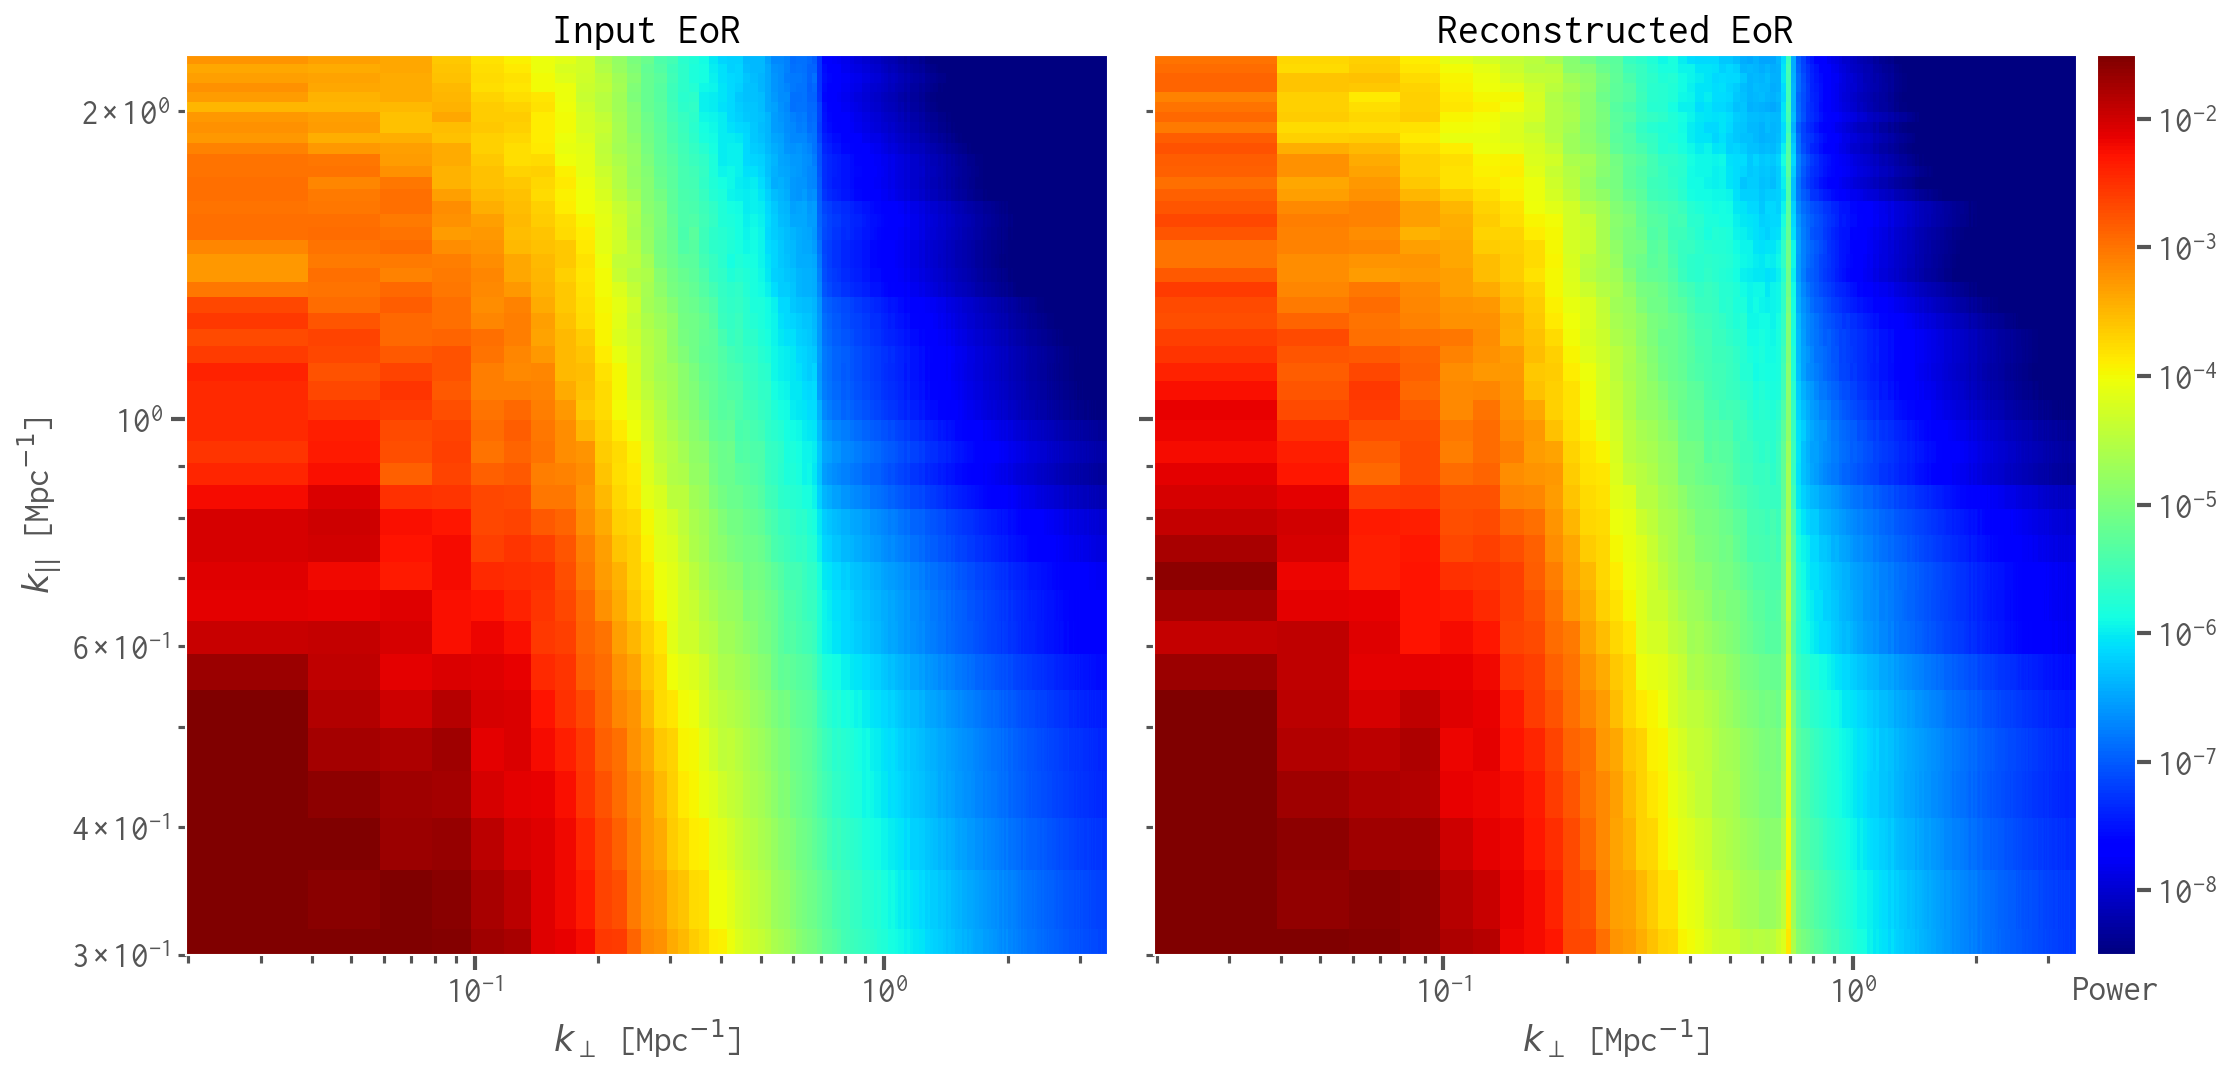
\includegraphics[width=\textwidth]{cdae-eor-ps-comp}
  \bicaption[输入的 EoR 信号和 CDAE 重建的 EoR 信号之间的二维功率谱对比]{%
    TODO...
  }{%
    Comparison of two-dimensional power spectra between the input (the left
    panel) and reconstructed (the right panel) EoR signals.
  }
  \label{fig:cdae-eor-ps}
\end{figure}

Since the test set $S_{\R{test}}$ is derived from the whole image cubes
$\left( C_{\R{eor}}^{(2)}, C_{\R{fg}}^{(2)} \right)$, we are able to create
complete images of the reconstructed EoR signal and calculate the
corresponding power spectrum.
Taking the input and reconstructed EoR images at the central frequency of
\SI{158}{\MHz} as an example (\autoref{fig:cdae-eor-img}), the reconstructed EoR
signal exhibits almost identical structures and amplitudes as the input EoR
signal.
We note that the reconstructed EoR image has weak but detectable redundant
ripples on scales of about 10 pixels (i.e., \SI{\sim 200}{\arcsecond}),
which are associated with the excision of the $n_{\R{ex}} = 6$ lowest
Fourier frequencies in data preprocessing (\autoref{sec:preprocessing}).
In addition, we calculate the two-dimensional power spectra from the image
cubes of the input and reconstructed EoR signals (\autoref{fig:cdae-eor-ps}).
It illustrates that the trained CDAE well recovers the EoR signal on all
covered scales except for a very thin stripe region at
$\kperp \approx \SI{0.7}{\per\Mpc}$, where extra powers are generated
by the aforementioned ripples in the reconstructed EoR images.
We also note that there is a barely visible line at
$\kperp \approx \SI{0.1}{\per\Mpc}$ in both power spectra, which is
caused by the boundary effect of Fourier transforming the finite frequency
band.

The results clearly demonstrate that the trained CDAE is able to accurately
reconstruct the EoR signal, overcoming the complicated beam effects.
The achieved excellent performance of the CDAE can be mainly attributed
to the architecture of stacking multiple convolutional layers, which
implements a powerful feature extraction technique by hierarchically
combining the basic features learned in each layer to build more and
more sophisticated features \cite{leCun2015}.
Combined with the flexibility provided by the \num{53569} trainable
parameters, the CDAE, after being well trained, can intelligently learn a
model that is optimised to accurately separate the faint EoR signal
\cite{domingos2012}.

%---------------------------------------------------------------------
\subsection{进一步验证}

With the purpose of further validating that the trained CDAE has actually
learned the useful features of the EoR signal, we employ the occlusion
method \cite{zeiler2014} to visualise the sensitivity of the trained CDAE
to the different part of the input data.
At each time, we occlude three adjacent elements of every input
$\B{x}$ in the validation set $S_{\R{val}}$, and then measure the CDAE's
sensitivity to the occluded part, which is calculated as the
occlusion-induced performance loss, i.e.,
\begin{equation}
  \label{eq:perf-loss}
  s = \frac{1}{N_{\R{val}}} \sum_{i=1}^{N_{\R{val}}} \left[
      \rho\left(\B{r}^{(i)}_{\R{eor}}, \B{x}^{(i)}_{\R{eor}}\right) -
      \rho\left(\B{R}^{(i)}_{\R{eor}}, \B{x}^{(i)}_{\R{eor}}\right)
    \right] ,
\end{equation}
where
$N_{\R{val}}$ is the number of data points in the validation set,
$\B{x}^{(i)}_{\R{eor}}$ is the input EoR signal, and
$\B{r}^{(i)}_{\R{eor}}$ and $\B{R}^{(i)}_{\R{eor}}$ are the reconstructed
EoR signals without and with applying the occlusion, respectively.
By varying the occlusion part of the input data and calculating the
sensitivities, we obtain the CDAE's sensitivity distribution ($\B{s}$) to
every part of the input data, as shown in \autoref{fig:occ-fgeor}, where
the root-mean-square amplitudes of the foreground emission
($\B{y}_{\R{fg}}$) and the EoR signal ($\B{y}_{\R{eor}}$) are also plotted.
We find that the sensitivity distribution is more correlated with the EoR
signal [$\rho(\B{s}, \B{y}_{\R{eor}}) = 0.742$] than the foreground
[$\rho(\B{s}, \B{y}_{\R{fg}}) = 0.562$].
This verifies that the trained CDAE has learned useful features of the EoR
signal to distinguish it from the foreground emission and thus becomes more
sensitive to the data parts of higher signal-to-noise ratio.

\begin{figure}[htp]
  \centering
  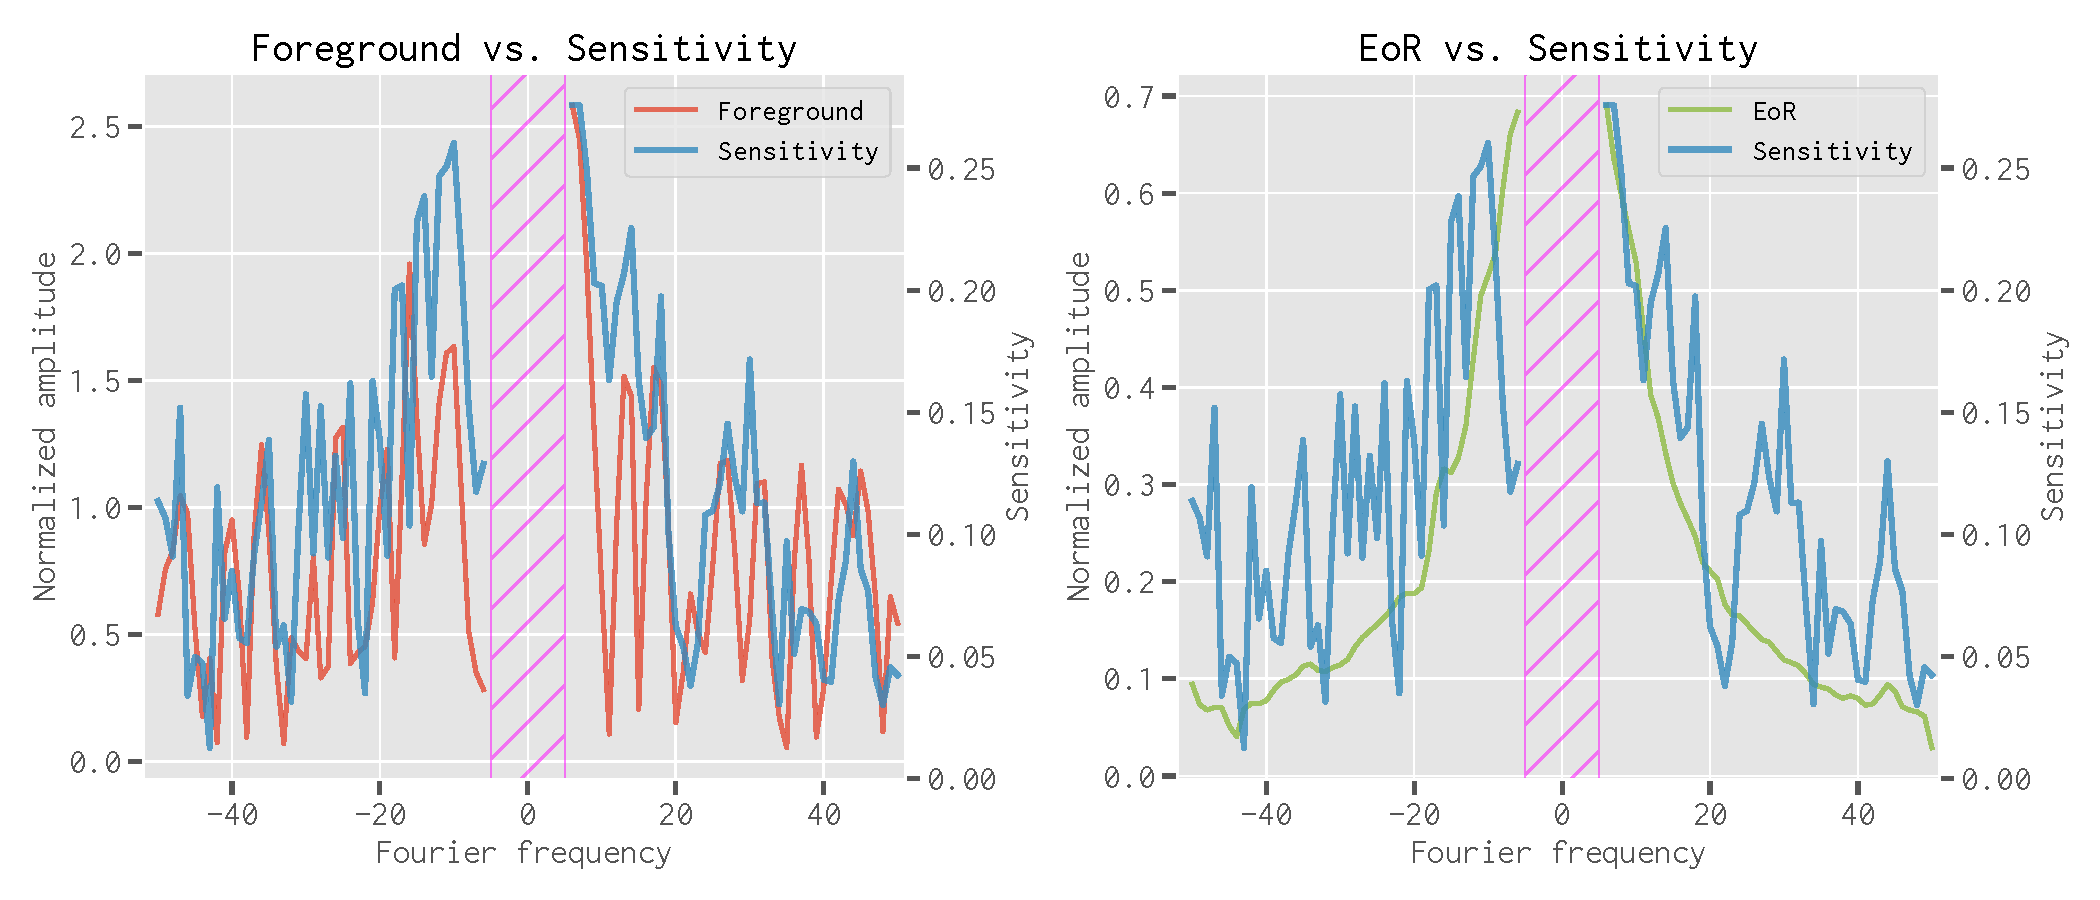
\includegraphics[width=\textwidth]{occlusion-fgeor}
  \bicaption[CDAE 对输入数据的灵敏度分布]{%
    TODO...
  }{%
    The CDAE's sensitivity distribution $\B{s}$ (the blue lines in both
    panels) obtained by applying the occlusion method.
    We also plot the root-mean-square amplitudes of the foreground emission
    ($\B{y}_{\R{fg}}$, the red line in the left panel) and the EoR signal
    ($\B{y}_{\R{eor}}$, the green line in the right panel).
    The sensitivity distribution $\B{s}$ is more correlated with the EoR
    signal [$\rho(\B{s}, \B{y}_{\R{eor}}) = 0.742$] than the foreground
    [$\rho(\B{s}, \B{y}_{\R{fg}}) = 0.562$].
  }
  \label{fig:occ-fgeor}
\end{figure}


%=====================================================================
\section{讨论}

TODO

%---------------------------------------------------------------------
\subsection{为什么使用 Fourier 变换预处理数据?}
\label{sec:why-ft}

We perform another experiment using the same CDAE architecture,
datasets, and data preprocessing steps, but without
applying the FT as depicted in \autoref{sec:preprocessing}.
After training the CDAE in the same way as described in
\autoref{sec:cdae-results}, the correlation coefficient between the
reconstructed and input EoR signals evaluated on the test set
$S_{\R{test}}$ reaches only $\bar{\rho}_{\R{noft}} = \num{0.628 +- 0.167}$,
which indicates a significantly worse performance compared to the case with
FT applied.
As presented in \autoref{fig:cdae-train-noft}, the training loss decreases more
slowly and converges after about 100 epochs.
We also find that the training process is slightly unstable given the small
spikes on the curves of both the loss and correlation coefficient.
These indicate that it is beneficial to preprocess the
dataset by applying the FT along the frequency dimension, because the
EoR signal and the foreground emission become more distinguishable
in the Fourier domain, where the fluctuating EoR signal concentrates on
larger Fourier modes while the spectral-smooth foreground emission
distributes mainly on smaller Fourier modes \cite{parsons2012}.

\begin{figure}[htp]
  \centering
  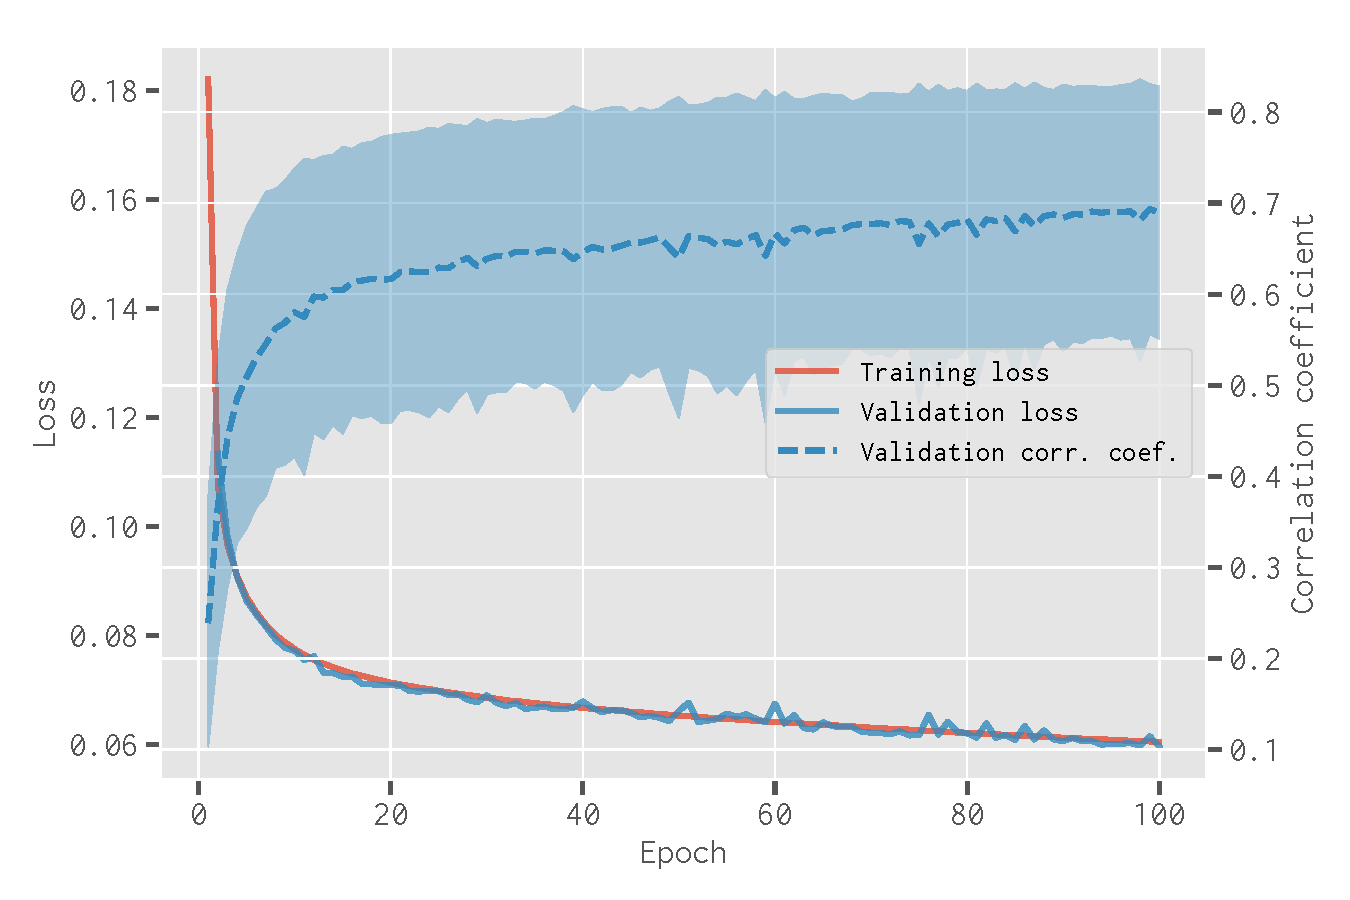
\includegraphics[width=\textwidth]{cdae-train-noft}
  \bicaption[在未经 Fourier 变换预处理的数据集上训练 CDAE 得到的结果]{%
    TODO... \autoref{fig:cdae-train}
  }{%
    Same as Fig.~\ref{fig:cdae-train} but for the case that the data are
    preprocessed without applying the FT.
  }
  \label{fig:cdae-train-noft}
\end{figure}


%---------------------------------------------------------------------
\subsection{与传统方法的对比}

A variety of methods have been proposed to remove the foreground
contamination with the aim of revealing the faint EoR signal.
These methods can be broadly classified into two categories:
(1) parametric methods that apply a parametric model (e.g., a low-degree
polynomial) to fit and remove the foreground emission
\cite{wang2006,jelic2008,liu2009fgrm,wang2013,bonaldi2015};
(2) non-parametric methods, which do not assume a specific parametric model
for the foreground emission but exploit the differences between the
foreground emission and the EoR signal (e.g., their different spectral
features) to separate them
\cite{harker2009,chapman2012,chapman2013,gu2013,mertens2018}.

In order to further demonstrate the performance of our method, we compare
it to two representative traditional methods:
the polynomial fitting method \cite{wang2006} and
the continuous wavelet transform (CWT) method \cite{gu2013}.
The polynomial fitting method is the best representative of the parametric
methods because it is widely used due to its simplicity and robustness
\cite{jelic2008,liu2009ps,pritchard2010}
and has been compared to various other foreground removal methods
\cite{harker2009,alonso2015,chapman2015}.
Among the non-parametric category, the CWT method is chosen since it
performs similarly well as other non-parametric methods, such as the
Wp smoothing method \cite{harker2009} and the generalized morphological
component analysis method \cite{chapman2013},
meanwhile it is faster and simpler \cite{gu2013,chapman2015}.

With the polynomial fitting method,
a low-degree polynomial is fitted along the frequency dimension for each
sky pixel in the image cube of the total emission (i.e.,
$C_{\R{tot}} = C_{\R{eor}} + C_{\R{fg}}$).
Then by subtracting the fitted smooth component, which is regarded as
the foreground emission, the EoR signal is expected to be uncovered.
Using the same image cubes
$\left( C_{\R{eor}}^{(2)}, C_{\R{fg}}^{(2)} \right)$
simulated in \autoref{sec:cdae-dataset},
we have tested polynomials of the degree from 2 (quadratic) to
5 (quintic), and find that the quartic polynomial (degree of 4)
can give the best result.
However, the correlation coefficient calculated for the separated EoR
signal in such a case is only
$\bar{\rho}_{\R{poly}} = \num{0.296 +- 0.121}$,
which indicates that the polynomial fitting method performs poorly in
removing the foreground emission.

The CWT method works based on the same assumption as other foreground
removal methods that the foreground emission is spectrally smooth while the
EoR signal fluctuates rapidly along the frequency dimension.
After applying the CWT, the foreground emission and the EoR signal locate
at different positions in the wavelet space because of their different
spectral scales.
Therefore, the foreground emission can be easily separated from the EoR
signal and be removed \cite{gu2013}.
For each sky pixel, the spectrum of the total emission is transformed into
the wavelet space by applying the CWT with the Morlet wavelet function.
In the wavelet space, after identifying and removing the coefficients that
are mainly contributed by the foreground emission, the remaining
coefficients are transformed back to the frequency space to obtain the
spectrum with the foreground emission removed, which is expected to be the
EoR signal.
By evaluating on the same dataset
$\left( C_{\R{eor}}^{(2)}, C_{\R{fg}}^{(2)} \right)$,
we have tuned the method parameters (minimum scale $s_{\R{min}}$, maximum
scale $s_{\R{max}}$, number of scales $n_s$, and cone of influence $c_i$)
and adopt $s_{\R{min}} = 7.4$, $s_{\R{max}} = 50.0$, $n_s = 50$, and
$c_i = 1.6$ to obtain the relatively best performance, which is, however,
only $\bar{\rho}_{\R{cwt}} = \num{0.198 +- 0.160}$.
We note that the CWT method performs slightly worse than the polynomial
fitting method, which is different from the comparison in \citet{gu2013}.
This may be caused by the more serious boundary effect since our simulated
data have a narrower bandwidth and coarser frequency resolution than those
of \citet{gu2013}.

The main reason that both traditional foreground removal methods only
obtain remarkably inferior results is that the smoothness of the foreground
spectra is seriously damaged by the frequency-dependent beam effects, which
cause rapid fluctuations of strength the same order as the EoR signal on
the originally smooth foreground spectra [\autoref{fig:cdae-simdata}(b)].
As a result, the foreground spectra complicated by the beam effects cannot
be well fitted by a low-degree polynomial and have more similar spectral
scales as the EoR signal.
In consequence, both methods are unable to well model the complicated
foreground spectra and thus have great difficulties in removing them.
On the contrary, given its data-driven nature and powerful feature
extraction capabilities, the CDAE is able to distil knowledge from the
training data and learns the features to distinguish the EoR signal from
the fluctuations arising from the beam effects.
Hence, the CDAE achieves superior performance in separating the EoR signal.


%=====================================================================
\section{小结}

The frequency-dependent beam effects of interferometers can cause
rapid fluctuations along the frequency dimension,
which damage the smoothness of the foreground spectra and prevent
traditional foreground removal methods from uncovering the EoR signal.
Given the difficulties in crafting practicable models to overcome the
complicated beam effects, methods that can intelligently learn tailored
models from the data seem more feasible and appealing.
To this end, we have proposed a deep-learning-based method that uses
a 9-layer CDAE to separate the EoR signal.
The CDAE has been trained on the simulated SKA images and has achieved
excellent performance.
We conclude that the CDAE has outstanding ability to overcome the
complicated beam effects and accurately separate the faint EoR signal,
exhibiting the great potential of deep-learning-based methods
to play an important role in the forthcoming EoR experiments.

本章内容已发表于 \mnras{} (MNRAS)\reviewornot{}{\cite{li.cdae}}.


%% EOF
